\chapter{Performance experiments}
Using a machine with an AMD Ryzen 5 3600 CPU @ 3.7GHz and sufficient 3200MHz memory we conduct several experiments with different inputs and setting. The results are shown in Tables \ref{tab:iterator-performance} through \ref{tab:pruning-performance-big}. 

For source graph-target graph pairs without a present vertex disjoint subgraph homeomorphism we consistently use the G(n, M) Erdős–Rényi random graph model.

Since vertex disjoint subgraph homeomorphisms are rare in random graphs, we construct source graph-target graph pairs with a present vertex disjoint subgraph homeomorphism a different way. First, wegenerating a random source graph using the use the G(n, M) Erdős–Rényi random graph model. Then we add vertices: with a 50\% probability we intersect a random existing edge with each new vertex and with 50\% probability we add it outside the existing graph. Then we add edges: while the vertices added outside the source graph have less-than-average degree we add uniformly sampled edges that include them; afterwards we add uniformly sampled random edges.

Firstly, we compare the different methods of path iteration. The time taken to explore the entire search tree (without homeomorphism) gives an indication of the overhead introduced by a pathiterator, not taking heuristic value into account. This comparison is shown in Figure \ref{fig:plotfailiterators}. The time taken for each path iteration method to find a homeomorphism where one exists is shown in Figure \ref{todo}. Here, the delay introduced caused by overhead may be offset by heuristic value.





%time to fail \ref{fig:plotfailiterators}
\begin{figure}
\centering
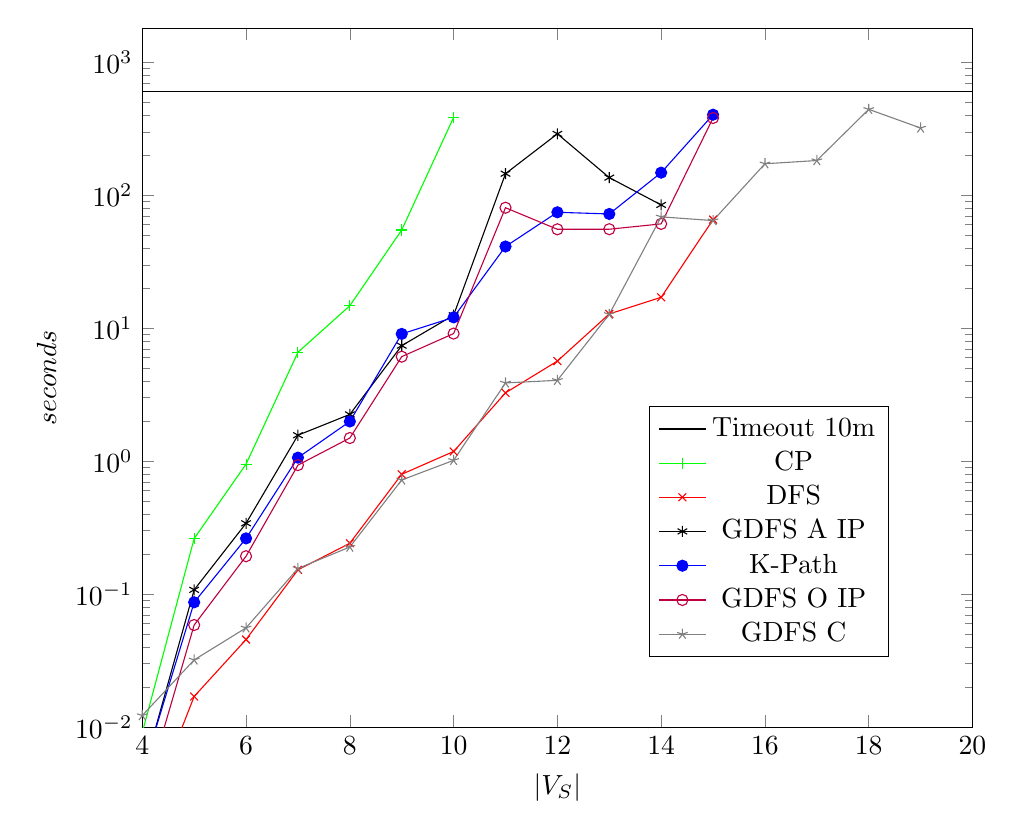
\begin{tikzpicture}
    \begin{axis}[
        xlabel=$|V_S|$,
        ylabel=$seconds$,
        ymin=0.01,
        ymode=log,
        xmin=4,
        xmax=20,
        legend style={at={(0.9,0.1)},anchor=south east},
        width=\textwidth,
    ]
    
\addplot[
        mark=none,
        black,
    ] plot coordinates {
        (4,600)
        (20,600)
};
    \addlegendentry{Timeout 10m}    
    
    
    \addplot[
        mark=+,
        green,
    ] plot coordinates {
        (4,0.009108628025032595) 
        (5,0.2620836802188065) 
        (6,0.9503740113943355)
        (7,6.596783503767442) 
        (8,14.764050718975609) 
        (9,54.765670739272736)
        (10,385.16296629500005) 
};
    \addlegendentry{CP}
    
    
    
    \addplot[
        mark=x,
        red,
    ] plot coordinates {
        (4,0.001716029672925713)
        (5,0.01702360071809101) 
        (6,0.04561513035914958) 
        (7,0.15251165322667018) 
        (8,0.24155461744973755) 
        (9,0.797513732268617) 
        (10,1.1835030509211046) 
        (11,3.2680702187065216)
        (12,5.661746851933962) 
        (13,12.798846733085105)
        (14,17.096358927307694)
        (15,65.64831186045454)
};
    \addlegendentry{DFS}
    
    
    
    \addplot[
        mark=asterisk,
        black,
    ] plot coordinates {
        (4,0.0043272421728668435) 
        (5,0.1078318674295203) 
        (6,0.3413335015273159)
        (7,1.5682172603423914)
        (8,2.249343766891791) 
        (9,7.395351140134146)
        (10,12.526694290867926)
        (11,145.27286338419998) 
        (12,289.503897899)
        (13,135.6942000877143) 
        (14,84.56603693766665)
};
    \addlegendentry{GDFS A IP}
    
    
    \addplot[
        mark=*,
        blue,
    ] plot coordinates {
        (4,0.004513287361457468) 
        (5,0.08689765890565003)
        (6,0.26278218619322824)
        (7,1.0640096504880734) 
        (8,1.9899295945868851)
        (9,9.064827074119401)
        (10,12.07097279138)
        (11,41.171574928875)
        (12,74.45223459277778)
        (13,72.3320726255)
        (14,147.87316945775) 
        (15,403.442499958)
};
    \addlegendentry{K-Path}
    
    \addplot[
        mark=o,
        purple,
    ] plot coordinates {
        (4,0.0027085184446120963) 
        (5,0.05864821291835853) 
        (6,0.19300624213070725) 
        (7,0.9348330173258064)
        (8,1.4939211758271604)
        (9,6.113139861699029)
        (10,9.11535311513433) 
        (11,80.54225475566666)
        (12,55.450854962)
        (13,55.5386134715)
        (14,60.892068884249994) 
        (15,381.159786211)
};
    \addlegendentry{GDFS O IP}
    
    
    \addplot[
        mark=star,
        gray,
    ] plot coordinates {
        (4,0.012242439615384614) 
        (5,0.032056864899625934) 
        (6,0.05582594232351259) 
        (7,0.15618683271269063) 
        (8,0.22630326749716662)
        (9,0.7229805422695548)
        (10,1.0152932454602368)
        (11,3.8780944653607596)
        (12,4.058766762371621)
        (13,12.724517174693878)
        (14,68.79296791008333)
        (15,64.49375942241666)
        (16,172.4802085922)
        (17,182.4329892165)
        (18,442.59586222949997)
        (19,320.441386005)
};
    \addlegendentry{GDFS C}
    \end{axis}
    \end{tikzpicture}
    \caption{A comparison of the speed of path iterators on directed graphs without a vertex disjoint subgraph homeomorphism. The time taken is measured of exploring the entire search tree without pruning or contraction and ``refuse longer paths" enabled. The source graph has average degree $3.0$ and the random target graph has $50\%$ more vertices and average degree $4.0$.}
    \label{fig:plotfailiterators}
\end{figure}


%time to succeed \ref{fig:plotsucceediterators} TODO: run 10m each
\begin{figure}
\centering
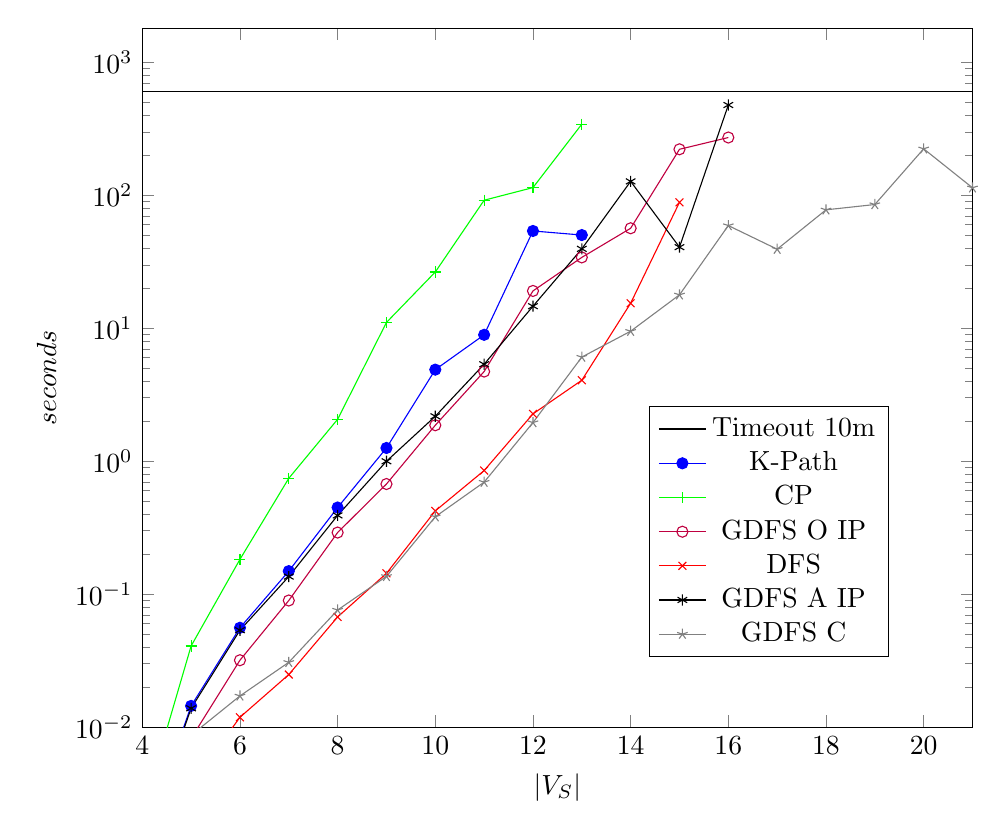
\begin{tikzpicture}
    \begin{axis}[
        xlabel=$|V_S|$,
        ylabel=$seconds$,
        ymin=0.01,
        ymode=log,
        xmin=4,
        xmax=21,
        legend style={at={(0.9,0.1)},anchor=south east},
        width=\textwidth,
    ]
    
    \addplot[
        mark=none,
        black,
    ] plot coordinates {
        (4,600)
        (21,600)
};
    \addlegendentry{Timeout 10m}


\addplot[
        mark=*,
        blue,
        error bars/.cd, y dir=both, y explicit,
    ] plot coordinates {
        (4,0.0012667032822330576)
        (5,0.014450939583729977)
        (6,0.05591708867636635)
        (7,0.14911566497364495)
        (8,0.44854427304185357)
        (9,1.257458328264463)
        (10,4.882261796422765)
        (11,8.92112126069014)
        (12,53.879064942750006)
        (13,50.1927055715)
};
    \addlegendentry{K-Path}
    
    \addplot[
        mark=+,
        green,
        error bars/.cd, y dir=both, y explicit,
    ] plot coordinates {
        (4,0.0022598064731390965)
        (5,0.040788492474074574)
        (6,0.18285989427787933)
        (7,0.7438714740483271)
        (8,2.0661439080927835)
        (9,11.051631589785714)
        (10,26.467970115956522)
        (11,91.75283437071428)
        (12,114.154734211)
        (13,342.4216391745)
};
    \addlegendentry{CP}
    
    
    \addplot[
        mark=o,
        purple,
        error bars/.cd, y dir=both, y explicit,
    ] plot coordinates {
        (4,7.913821003220384E-4)
        (5,0.008231382983722117)
        (6,0.031882214566006595)
        (7,0.08963993490432053)
        (8,0.29087998969535783)
        (9,0.6738117268754134)
        (10,1.8639315102639753)
        (11,4.723388754421875)
        (12,19.076032830888888)
        (13,34.09402854616666)
        (14,56.448447976636366)
        (15,221.585912108)
        (16,271.705023368)
};
    \addlegendentry{GDFS O IP}
    
    
    \addplot[
        mark=x,
        red,
        error bars/.cd, y dir=both, y explicit,
    ] plot coordinates {
        (4,5.262049048412901E-4)
        (5,0.0037078367276320813)
        (6,0.011864989818313664)
        (7,0.024878632873617693)
        (8,0.06746086448666291)
        (9,0.1434635451083732)
        (10,0.42305252119181946)
        (11,0.8507154702662889)
        (12,2.2694573458389513)
        (13,4.062910206266234)
        (14,15.418462455714286)
        (15,88.48300721233333)
};
    \addlegendentry{DFS}
    
    
    \addplot[
        mark=asterisk,
        black,
        error bars/.cd, y dir=both, y explicit,
    ] plot coordinates {
        (4,0.0012375753780820582)
        (5,0.01386437069184402)
        (6,0.053590561273019845)
        (7,0.1357242449547409)
        (8,0.3913462516747066)
        (9,0.9992033137657806)
        (10,2.177200933823741)
        (11,5.359800497321429)
        (12,14.644324665268291)
        (13,39.5231686368125)
        (14,127.138527012)
        (15,40.69748180766667)
        (16,477.083996688)
};
    \addlegendentry{GDFS A IP}
    
    
    \addplot[
        mark=star,
        gray,
        error bars/.cd, y dir=both, y explicit,
    ] plot coordinates {
        (4,0.005644702207616498)
        (5,0.008692270720925143)
        (6,0.017174057391094375)
        (7,0.03073833753675828)
        (8,0.07604849509162437)
        (9,0.13615389069436876) 
        (10,0.38220422819426747)
        (11,0.6959524782169374)
        (12,1.95247773692233)
        (13,6.06748104474) 
        (14,9.499085503648649) 
        (15,17.829571026735294) 
        (16,59.15707016833334) 
        (17,39.30442401336364) 
        (18,77.68409019719999) 
        (19,85.162749429) 
        (20,223.46494652625)
        (21,113.76846415325) 
};
    \addlegendentry{GDFS C}


   
    \end{axis}
    \end{tikzpicture}
    \caption{A comparison of the speed of path iterators on directed graphs with a vertex disjoint subgraph homeomorphism. The time taken is measured of exploring the entire search tree without pruning or contraction and ``refuse longer paths" enabled. The source graph has average degree $3.0$ and the random target graph has $50\%$ more vertices and average degree $4.0$.}
    \label{fig:plotsucceediterators}
\end{figure}



%contraction times \ref{fig:contractionsmall} timeout 30m
\begin{figure}
\centering
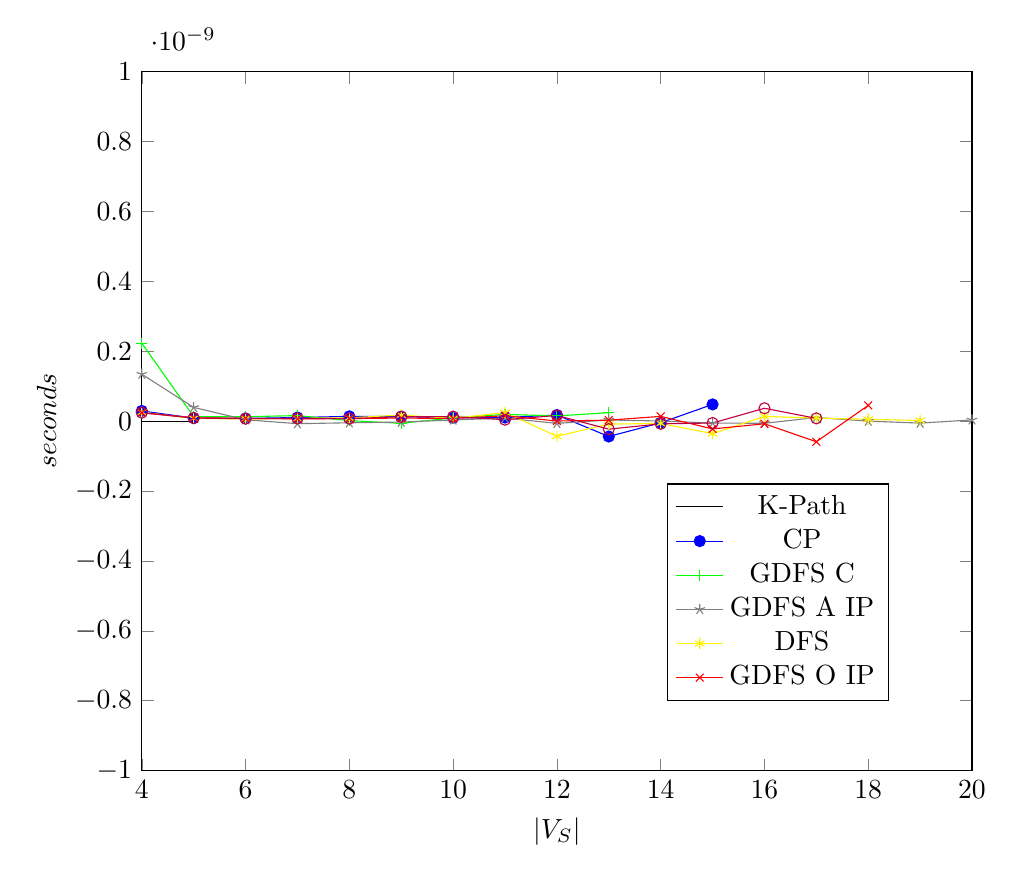
\begin{tikzpicture}
    \begin{axis}[
        xlabel=$|V_S|$,
        ylabel=$seconds$,
        ymin=-0.000000001,
        ymax=0.000000001,
        xmin=4,
        xmax=20,
        legend style={at={(0.9,0.1)},anchor=south east},
        width=\textwidth,
    ]


\addplot [mark=none, black] {0.0};



\addplot[
        mark=*,
        blue,
    ] plot coordinates {
        (4,2.932140993814181E-11)
        (5,8.7720080091192E-12)
        (6,7.959205083828377E-12)
        (7,1.0516842935321274E-11)
        (8,1.3846681720649775E-11)
        (9,1.3278493322591943E-11)
        (10,9.431772188690199E-12)
        (11,1.0427742369645348E-11)
        (12,1.762989368085995E-11)
        (13,-4.37768516655734E-11)
        (14,-4.511212917791829E-12)
        (15,4.8026201083270074E-11)
};
    \addlegendentry{K-Path}
    
    
    
\addplot[
        mark=+,
        green,
    ] plot coordinates {
        (4,2.2332244791963868E-10)
        (5,1.2894586030492787E-11)
        (6,1.2739181300796536E-11)
        (7,1.6017815465222444E-11)
        (8,1.6604858933035923E-12)
        (9,-6.059090199426299E-12)
        (10,9.39594395535824E-12)
        (11,1.9454408356813372E-11)
        (12,1.506393331670645E-11)
        (13,2.4343296338245503E-11)
};
    \addlegendentry{CP}
    

\addplot[
        mark=star,
        gray,
    ] plot coordinates {
        (4,1.3449236191090652E-10)
        (5,3.9424461507144745E-11)
        (6,4.123997948788519E-12)
        (7,-7.124749000038612E-12)
        (8,-4.550093751058444E-12)
        (9,-2.557899737322365E-12)
        (10,3.4839846092196797E-12)
        (11,8.924880334219604E-12)
        (12,-6.3266559625812015E-12)
        (13,3.4830158320769448E-12)
        (14,4.471491114813807E-13)
        (15,-5.3583849118332295E-12)
        (16,-6.032475121829378E-12)
        (17,1.0580563826445032E-11)
        (18,2.4921100870856105E-13)
        (19,-5.51069485408738E-12)
        (20,3.6745570894507475E-12)
};
    \addlegendentry{GDFS C}
    
   
   
\addplot[
        mark=asterisk,
        yellow,
    ] plot coordinates {
        (4,2.5817014120104498E-11)
        (5,7.588652938149603E-12)
        (6,6.678659103281653E-12)
        (7,7.795817566846849E-12)
        (8,9.740183930072732E-12)
        (9,1.7547084454832595E-11)
        (10,8.007714438420118E-12)
        (11,2.472236632832395E-11)
        (12,-4.3069129019126646E-11)
        (13,-8.286425287724539E-12)
        (14,-6.52925051744273E-12)
        (15,-3.567912623592618E-11)
        (16,1.3722965201731106E-11)
        (17,9.008197187185096E-12)
        (18,5.332941508324916E-12)
        (19,2.0033625302170086E-12)
};
    \addlegendentry{GDFS A IP}
    
    \addplot[
        mark=x,
        red,
    ] plot coordinates {
        (4,2.404005357065415E-11)
        (5,9.847114925286539E-12)
        (6,8.222595522624967E-12)
        (7,6.694101448821747E-12)
        (8,7.50354643777528E-12)
        (9,8.966580808443709E-12)
        (10,7.694811181400364E-12)
        (11,1.550304446686373E-11)
        (12,5.195414819744207E-13)
        (13,2.96892886474811E-12)
        (14,1.3809535325944459E-11)
        (15,-2.2146582030819945E-11)
        (16,-7.43249518357636E-12)
        (17,-5.879366264527795E-11)
        (18,4.52192973530775E-11)
};
    \addlegendentry{DFS}
    
    \addplot[
        mark=o,
        purple,
    ] plot coordinates {
        (4,2.4281869530195394E-11)
        (5,8.94728269970603E-12)
        (6,7.1701111074078675E-12)
        (7,7.875692218417016E-12)
        (8,7.438503763179787E-12)
        (9,1.2660715198450901E-11)
        (10,1.3068978206401108E-11)
        (11,4.242523937867266E-12)
        (12,1.6340262407110805E-11)
        (13,-2.2798295806268762E-11)
        (14,-7.487971797449773E-12)
        (15,-5.214674853044758E-12)
        (16,3.6968087345378095E-11)
        (17,8.07749651664158E-12)
};
    \addlegendentry{GDFS O IP}



    \end{axis}
    \end{tikzpicture}
    \caption{Relative performance of contraction-enabled vertex disjoint subgraph homeomorphism compared to contraction-disabled for different path iteration methods. Mind the scale of the vertical axis ($10^{-9}$)}
    \label{fig:contractionsmall}
\end{figure}









\begin{table}[ht]
\centering
\begin{tabular}{|l|l|l|l|l|l|l|}
\hline
\textbf{Path iteration} &
  \textbf{Its/success} &
  \textbf{Time/iteration} &
  \textbf{time/success} &
  \textbf{stdev} &
  \textbf{time/fail} &
  \textbf{stdev} \\ \hline
K-Path        &  &  &  &  &  &  \\ \hline
DFS           &  &  &  &  &  &  \\ \hline
Greedy DFS    &  &  &  &  &  &  \\ \hline
Control point &  &  &  &  &  &  \\ \hline
\end{tabular}
\caption{Performance of different path iteration methods on random source graphs of size $|V|\in \{8..12\}$ with edge density 3.0 and random target graphs of size $|V|\in \{15..20\}$ with edge density 4.0. ``refuse unnecessarily long paths" and contraction are enabled and parallel all-different pruning is used.}
\label{tab:iterator-performance}
\end{table}




\begin{table}[ht]
\centering
\begin{tabular}{|l|l|l|l|l|l|l|}
\hline
\textbf{Path iteration} &
  \textbf{Its/success} &
  \textbf{Time/iteration} &
  \textbf{time/success} &
  \textbf{stdev} &
  \textbf{time/fail} &
  \textbf{stdev} \\ \hline
K-Path        &  &  &  &  &  &  \\ \hline
DFS           &  &  &  &  &  &  \\ \hline
Greedy DFS    &  &  &  &  &  &  \\ \hline
Control point &  &  &  &  &  &  \\ \hline
\end{tabular}
\caption{Performance of different path iteration methods on random source graphs of size $|V|\in \{1..5\}$ with edge density 3.0 and a square of four ECP5 logic tiles as target graph. ``refuse unnecessarily long paths" and contraction are enabled and parallel all-different pruning is used.}
\label{tab:iterator-performance}
\end{table}

\begin{table}[ht]
\centering
\begin{tabular}{|l|l|l|l|l|l|}
\hline
\textbf{Source graph size} & \textbf{Target graph size} & \textbf{K-Path} & \textbf{DFS} & \textbf{Greedy DFS} & \textbf{CP} \\ \hline
$|V|=5$, $|E|=10$          & $|V|=8$, $|E|=15$          & -30.0\%                     & +10.0\%          &  -20.0\%                      & -17.0\%               \\ \hline
&&&&&\\\hline
&&&&&\\\hline
&&&&&\\\hline
&&&&&\\\hline
&&&&&\\\hline
&&&&&\\\hline
                           & single ECP5 tile         &                           &                &                        &                \\ \hline
                                                      & square of ECP5 tiles         &                           &                &                        &                \\ \hline
\end{tabular}
\caption{The performance benefit (seconds) of the `refuse unnecessarily long paths' setting on random source graphs and random target graphs.}
\label{tab:refuselongerpaths-performance}
\end{table}



\begin{table}[ht]
\centering
\begin{tabular}{|l|l|l|l|l|l|}
\hline
\textbf{Source graph size} & \textbf{Target graph size} & \textbf{K-Path} & \textbf{DFS} & \textbf{Greedy DFS} & \textbf{CP} \\ \hline
$|V|=5$, $|E|=10$          & $|V|=8$, $|E|=15$          & -30.0\%                     & +10.0\%          &  -20.0\%                      & -17.0\%               \\ \hline
&&&&&\\\hline
&&&&&\\\hline
&&&&&\\\hline
&&&&&\\\hline
&&&&&\\\hline
&&&&&\\\hline
                           & single ECP5 tile         &                           &                &                        &                \\ \hline
                                                      & square of ECP5 tiles         &                           &                &                        &                \\ \hline
\end{tabular}
\caption{The performance benefit (seconds) of contraction on random source graphs and random target graphs.}
\label{tab:contraction-performance}
\end{table}




% Please add the following required packages to your document preamble:
% \usepackage{multirow}
\begin{table}[]
\begin{tabular}{|l|l|l|l|l|}
\hline
\textbf{Pruning strategy}      & \textbf{Filtering}               & \textbf{Application} & \textbf{Effect (+)} & \textbf{Effect (-)} \\ \hline
None                           &                                  &                      & +0.0\%              & +0.0\%              \\ \hline
\multirow{12}{*}{Zero domain}  & \multirow{3}{*}{Label/degree}    & Serial               &                     &                     \\ \cline{3-5} 
                               &                                  & Cached               &                     &                     \\ \cline{3-5} 
                               &                                  & Parallel             &                     &                     \\ \cline{2-5} 
                               & \multirow{3}{*}{Free neighbours} & Serial               &                     &                     \\ \cline{3-5} 
                               &                                  & Cached               &                     &                     \\ \cline{3-5} 
                               &                                  & Parallel             &                     &                     \\ \cline{2-5} 
                               & \multirow{3}{*}{M-reachability}  & Serial               &                     &                     \\ \cline{3-5} 
                               &                                  & Cached               &                     &                     \\ \cline{3-5} 
                               &                                  & Parallel             &                     &                     \\ \cline{2-5} 
                               & \multirow{3}{*}{N-reachability}  & Serial               &                     &                     \\ \cline{3-5} 
                               &                                  & Cached               &                     &                     \\ \cline{3-5} 
                               &                                  & Parallel             &                     &                     \\ \hline
\multirow{12}{*}{AllDifferent} & \multirow{3}{*}{Label/degree}    & Serial               &                     &                     \\ \cline{3-5} 
                               &                                  & Cached               &                     &                     \\ \cline{3-5} 
                               &                                  & Parallel             &                     &                     \\ \cline{2-5} 
                               & \multirow{3}{*}{Free neighbours} & Serial               &                     &                     \\ \cline{3-5} 
                               &                                  & Cached               &                     &                     \\ \cline{3-5} 
                               &                                  & Parallel             &                     &                     \\ \cline{2-5} 
                               & \multirow{3}{*}{M-reachability}  & Serial               &                     &                     \\ \cline{3-5} 
                               &                                  & Cached               &                     &                     \\ \cline{3-5} 
                               &                                  & Parallel             &                     &                     \\ \cline{2-5} 
                               & \multirow{3}{*}{N-reachability}  & Serial               &                     &                     \\ \cline{3-5} 
                               &                                  & Cached               &                     &                     \\ \cline{3-5} 
                               &                                  & Parallel             &                     &                     \\ \hline
\end{tabular}
\caption{The performance effect (seconds) of different pruning methods with- and without Connectivity check (CC) and neighbour check (NC) on random source graphs of size $|V|\in \{8..12\}$ with edge density 3.0 and a square of four ECP5 times as target graph. Effect (+) denotes cases with some homeomorphism and Effect (-) denotes cases without a homemorphism.}
\label{tab:pruning-performance-small}
\end{table}



% Please add the following required packages to your document preamble:
% \usepackage{multirow}
\begin{table}[]
\begin{tabular}{|l|l|l|l|l|}
\hline
\textbf{Pruning strategy}      & \textbf{Filtering}               & \textbf{Application} & \textbf{Effect (+)} & \textbf{Effect (-)} \\ \hline
None                           &                                  &                      & +0.0\%              & +0.0\%              \\ \hline
\multirow{12}{*}{Zero domain}  & \multirow{3}{*}{Label/degree}    & Serial               &                     &                     \\ \cline{3-5} 
                               &                                  & Cached               &                     &                     \\ \cline{3-5} 
                               &                                  & Parallel             &                     &                     \\ \cline{2-5} 
                               & \multirow{3}{*}{Free neighbours} & Serial               &                     &                     \\ \cline{3-5} 
                               &                                  & Cached               &                     &                     \\ \cline{3-5} 
                               &                                  & Parallel             &                     &                     \\ \cline{2-5} 
                               & \multirow{3}{*}{M-reachability}  & Serial               &                     &                     \\ \cline{3-5} 
                               &                                  & Cached               &                     &                     \\ \cline{3-5} 
                               &                                  & Parallel             &                     &                     \\ \cline{2-5} 
                               & \multirow{3}{*}{N-reachability}  & Serial               &                     &                     \\ \cline{3-5} 
                               &                                  & Cached               &                     &                     \\ \cline{3-5} 
                               &                                  & Parallel             &                     &                     \\ \hline
\multirow{12}{*}{AllDifferent} & \multirow{3}{*}{Label/degree}    & Serial               &                     &                     \\ \cline{3-5} 
                               &                                  & Cached               &                     &                     \\ \cline{3-5} 
                               &                                  & Parallel             &                     &                     \\ \cline{2-5} 
                               & \multirow{3}{*}{Free neighbours} & Serial               &                     &                     \\ \cline{3-5} 
                               &                                  & Cached               &                     &                     \\ \cline{3-5} 
                               &                                  & Parallel             &                     &                     \\ \cline{2-5} 
                               & \multirow{3}{*}{M-reachability}  & Serial               &                     &                     \\ \cline{3-5} 
                               &                                  & Cached               &                     &                     \\ \cline{3-5} 
                               &                                  & Parallel             &                     &                     \\ \cline{2-5} 
                               & \multirow{3}{*}{N-reachability}  & Serial               &                     &                     \\ \cline{3-5} 
                               &                                  & Cached               &                     &                     \\ \cline{3-5} 
                               &                                  & Parallel             &                     &                     \\ \hline
\end{tabular}
\caption{The performance effect (seconds) of different pruning methods with- and without Connectivity check (CC) and neighbour check (NC) on random source graphs of size $|V|\in \{8..12\}$ with edge density 3.0 and a square of four ECP5 times as target graph. Effect (+) denotes cases with some homeomorphism and Effect (-) denotes cases without a homemorphism.}
\label{tab:pruning-performance-big}
\end{table}
